% Post-Quantum Cryptography Migration on DLTs — with notes for the Ethereum community
% Light repurpose of the BGIN GDC26 breakout deck
% (GDC26_PQC_Migration_DLTs_Slides.pdf, BGIN – Mitchell Travers & Shin'ichiro Matsuo, 3 Sep 2026).
% Slides 1-12 and 17-21 keep the original order and wording (DLT-generic). Light touches only:
% title/footer, a pointer on slide 2, the two diagrams that rendered blank in the original
% (slides 9, 10) drawn, venue/QR update on the last slide. Slides 13-16 are NEW:
% "Notes for the Ethereum community" on participating in the competition.
% Ethereum facts follow bgin-global/pqc-agility-competition main 86c780a (draft v0, nothing ratified).
% Build: latexmk -pdf GDC26_PQC_Migration_DLTs_Ethereum_Notes.tex
\documentclass[aspectratio=169,10pt]{beamer}
\usepackage[utf8]{inputenc}
\usepackage[T1]{fontenc}
\usepackage{helvet}
\renewcommand{\familydefault}{\sfdefault}
\usepackage{booktabs}
\usepackage{array}
\usepackage{graphicx}
\usepackage{fontawesome5}
\usepackage{tikz}
\usetikzlibrary{arrows.meta,positioning,calc}
\usepackage{qrcode}
\usepackage{hyperref}

% ---------- look: dark title bar, white body, grey footer (as in the original) ----------
\usetheme{default}
\definecolor{bar}{RGB}{25,25,29}
\definecolor{ink}{RGB}{35,35,40}
\definecolor{soft}{RGB}{110,110,118}
\definecolor{boxbg}{RGB}{242,242,244}
\definecolor{lane}{RGB}{225,227,232}
\definecolor{eth}{RGB}{72,82,140}
\definecolor{ethbg}{RGB}{232,234,246}
\setbeamercolor{normal text}{fg=ink}
\setbeamercolor{structure}{fg=bar}
\setbeamercolor{frametitle}{bg=bar,fg=white}
\setbeamercolor{block body}{bg=boxbg,fg=ink}
\setbeamercolor{eth body}{bg=ethbg,fg=ink}
\setbeamertemplate{navigation symbols}{}
\setbeamertemplate{itemize item}{\color{bar}\faAngleRight}
\setbeamertemplate{enumerate item}{\colorbox{bar}{\color{white}\scriptsize\insertenumlabel}}
\setbeamerfont{frametitle}{series=\bfseries,size=\large}
\setbeamertemplate{frametitle}{%
  \vskip-2pt\begin{beamercolorbox}[wd=\paperwidth,ht=8mm,dp=2.5mm,leftskip=6mm]{frametitle}%
  \usebeamerfont{frametitle}\insertframetitle\end{beamercolorbox}}
\setbeamertemplate{footline}{%
  \begin{beamercolorbox}[wd=\paperwidth,ht=5mm,dp=2mm,leftskip=6mm,rightskip=6mm]{normal text}%
  \tiny\color{soft}\raisebox{-1.2pt}{
\includegraphics[height=3.2mm]{bgin_mark.png}}\hspace{1.2mm}%
  GDC 2026 --- PQC Migration on DLTs \textperiodcentered{} with notes for the Ethereum community\hfill
  October 2026 / \insertframenumber\end{beamercolorbox}}
\newcommand{\takeaway}[1]{\par\vspace{1.5mm}{\small\color{bar}\faLink~\textbf{Takeaway:} #1}}
\newcommand{\lead}[1]{\begin{beamercolorbox}[wd=\textwidth,sep=2.5mm]{block body}\small #1\end{beamercolorbox}\par\vspace{2mm}}
\newcommand{\ethlead}[1]{\begin{beamercolorbox}[wd=\textwidth,sep=2.5mm]{eth body}\small #1\end{beamercolorbox}\par\vspace{2mm}}
\newcommand{\ethnote}[1]{\par\vspace{1.5mm}{\small\color{eth}\faEthereum~\textbf{For Ethereum:} #1}}
\newcommand{\pillar}[3]{\begin{minipage}[t]{#1}\colorbox{bar}{\parbox{\dimexpr\linewidth-2\fboxsep}{\color{white}\small\textbf{#2}}}\par\vspace{1mm}{\small #3}\end{minipage}}
\newcommand{\ethpillar}[3]{\begin{minipage}[t]{#1}\colorbox{eth}{\parbox{\dimexpr\linewidth-2\fboxsep}{\color{white}\small\textbf{#2}}}\par\vspace{1mm}{\small #3}\end{minipage}}
\hypersetup{colorlinks,urlcolor=bar,linkcolor=ink}

\begin{document}

% ---------------------------------------------------------------- 1 title
{\setbeamertemplate{footline}{}
\begin{frame}[plain,t]
  \begin{tikzpicture}[remember picture,overlay]
    \fill[bar] (current page.north west) rectangle ([yshift=-3.1cm]current page.north east);
    \node[anchor=north east,inner sep=0] at ([xshift=-7mm,yshift=-5mm]current page.north east){
\includegraphics[height=1.9cm]{bgin_logo.png}};
    \node[anchor=west,text=white,font=\Large\bfseries] at ([xshift=7mm,yshift=-1.55cm]current page.north west){Post-Quantum Cryptography Migration on DLTs};
    \node[anchor=west,text=white,font=\small,text width=11.2cm,align=left] at ([xshift=7mm,yshift=-2.45cm]current page.north west){Deployment, Agility \& Governance --- with notes for the Ethereum community on taking part in the competition};
    \node[anchor=west,font=\normalsize] at ([xshift=7mm,yshift=-4.5cm]current page.north west){BGIN -- Mitchell Travers \& Shin'ichiro Matsuo};
    \node[anchor=west,font=\small,text=soft] at ([xshift=7mm,yshift=-5.15cm]current page.north west){Global Digital Collaboration \textbar{} Geneva \textbar{} 2--3 September 2026};
    \node[anchor=west,font=\scriptsize,text=soft,text width=13cm,align=left] at ([xshift=7mm,yshift=-6.2cm]current page.north west){Ethereum community edition, October 2026 \textperiodcentered{} the GDC26 breakout deck plus four slides on Ethereum participation \textperiodcentered{} ecosystem-neutral: no chain and no scheme is endorsed};
  \end{tikzpicture}
\end{frame}}

% ---------------------------------------------------------------- 2 frame
\begin{frame}{Post-Quantum Cryptography Migration on DLTs}
  \lead{Wallets and credentials rely on long-lived cryptographic trust. NIST-standardized post-quantum cryptography is available. The work in this room is \textbf{deployment, crypto agility, and governance} --- not a new algorithm contest.}
  {\small\textbf{Co-organizers}}
  \begin{itemize}\small
    \item ISO
    \item Blockchain Group: BGIN, Blockchain Bundesverband e.V., Ethereum Climate Platform, LNet
    \item Linux Foundation Group: OpenWallet, Trust Over IP, LF Decentralized Trust
  \end{itemize}
  \ethnote{This is the deck presented at GDC26 in Geneva. Slides 13--16 are added for Ethereum client teams, researchers, wallet and L2 builders: where Ethereum sits in the competition, what gets measured, which rulings are still open, and how to take part.}
\end{frame}

% ---------------------------------------------------------------- 3 not another primitive
\begin{frame}{The Job Is Not to Pick Another Primitive}
  \lead{First PQC standards are in place (ML-KEM, ML-DSA, SLH-DSA). Re-running a competition inside this breakout would waste the hour.}
  {\small What still has no agreed playbook for public ledgers, wallets, and credentials:}
  \begin{itemize}\small
    \item How to stage a hybrid then a cutover when every node must agree on validity rules.
    \item How to keep verifying old signatures for as long as funds and archives remain live.
    \item How to rotate keys and addresses without stranding dormant accounts.
    \item How to tell a genuine PQ-ready stack from a screenshot.
  \end{itemize}
  \takeaway{Treat PQC as a multi-year systems and governance program, not a weekend library swap.}
\end{frame}

% ---------------------------------------------------------------- 4 not like TLS
\begin{frame}{Why This Stack Does Not Migrate Like TLS}
  \begin{center}\small
  \begin{tabular}{@{}p{6.2cm}p{7.3cm}@{}}\toprule
    \textbf{Enterprise PKI / TLS} & \textbf{Public DLT / wallets}\\ \midrule
    An operator can force a cutover & No single party can force consensus\\
    Cipher suites can be negotiated per session & Validity rules are global and sticky\\
    Certificates expire on a known clock & On-chain signatures must stay verifiable for decades\\
    Harvest-now, decrypt-later is mainly archival & Public keys often sit in the clear on-chain\\
    Evidence lives in a vendor report & ``PQ-ready'' claims need comparable measurement\\ \bottomrule
  \end{tabular}\end{center}
  \takeaway{A TLS playbook fails on three axes at once: decentralized upgrades, long-lived authenticity, and economic incentives.}
\end{frame}

% ---------------------------------------------------------------- 5 two halves
\begin{frame}{Two Halves of the Same 50 Minutes}
  \lead{Migration urgency is a function of resource estimates. Policy rooms keep hearing ``migrate now'' and ``decades away'' from different speakers. This breakout holds both halves in one place.}
  \pillar{0.48\textwidth}{Resource estimates}{What would actually be required to break widely used elliptic-curve signatures, under which assumptions, and with which honest error bars. No calendar marketing of a single Q-day.}\hfill
  \pillar{0.48\textwidth}{Migration and agility}{Hybrid signatures, staged activation, wallet and L2 impact, post-quantum ZKP where proofs are in the trust path, and MPC where key management takes the hit.}
  \takeaway{The estimates set the clock. The architecture sets whether the clock can be met without a rushed incident.}
\end{frame}

% ---------------------------------------------------------------- 6 exists / gap
\begin{frame}{What Already Exists --- and the Honest Gap}
  \begin{columns}[T]
    \begin{column}{0.48\textwidth}
      {\small\textbf{Already standardized}}
      \begin{itemize}\small
        \item NIST PQC primitives for KEM and signatures
        \item Hybrid patterns in adjacent Internet protocols
        \item National and industry migration handbooks for enterprise stacks
      \end{itemize}
    \end{column}
    \begin{column}{0.48\textwidth}
      {\small\textbf{Still missing for DLT}}
      \begin{itemize}\small
        \item Agreed migration requirements (correctness, long-term integrity, activation)
        \item Comparable benchmarks, not screenshots
        \item A governance path for dormant funds and multi-client stacks
      \end{itemize}
    \end{column}
  \end{columns}
  \par\vspace{2mm}
  {\small Triage axes that still need a first cut in this room: \textbf{protection lifetime}; \textbf{impact if broken}; \textbf{migration cost and dependencies}.}
  \takeaway{Do not invent a rival algorithm list. Write the DLT gap on top of NIST schemes.}
\end{frame}

% ---------------------------------------------------------------- 7 BGIN started
\begin{frame}{What BGIN Has Already Started}
  \lead{We are not starting from zero. IKP has been running crypto agility and PQC migration as a standing work item through recent Block meetings.}
  \begin{itemize}\small
    \item Meeting reports from Block 12 through Block 14 on transition, crypto agility, and PQC migration.
    \item A shared stance: NIST-standardized schemes only; no BGIN algorithm contest; no chain endorsement.
    \item Japan's government-hosted PQC migration prize, introduced on the next three slides, as one measurement path --- not as a second standard.
    \item Follow-on technical work at BGIN Block \#15 (October 2026), including dialogue with NIST.
  \end{itemize}
  \takeaway{GDC captures the gaps a 50-minute policy-and-practice room can name. Block 15 is where drafting continues.}
\end{frame}

% ---------------------------------------------------------------- 8 prize
\begin{frame}{Japan's PQC Migration Prize --- What It Is}
  \lead{A multi-year, internationally open prize competition on post-quantum migration for public blockchains. Hosted by the Japanese Government (METI/NEDO). BGIN coordinates internationally and runs a neutral evaluation testbed.}
  \begin{columns}[T]
    \begin{column}{0.48\textwidth}
      {\small\textbf{It is}}
      \begin{itemize}\small
        \item A push to accelerate and de-risk deployment of quantum-resistant signatures and advanced key management.
        \item Transparent, reproducible evaluation on a geographically distributed academic testbed (BSafe.network).
        \item A pipeline toward shared practice --- not a one-off ceremony.
      \end{itemize}
    \end{column}
    \begin{column}{0.48\textwidth}
      {\small\textbf{It is not}}
      \begin{itemize}\small
        \item Not a BGIN-owned contest. Japan hosts and funds the prize; BGIN coordinates and evaluates.
        \item Not a new-algorithm contest. Entries start from NIST-standardized schemes.
        \item Not chain endorsement, and not a single Q-day calendar claim.
      \end{itemize}
    \end{column}
  \end{columns}
  \takeaway{The hard problem on public chains is deployment, evaluation, and migration governance --- not selecting a new primitive.}
\end{frame}

% ---------------------------------------------------------------- 9 three lanes (drawn; blank in the original PDF)
\begin{frame}{Three Lanes and What Gets Evaluated}
  \begin{center}
  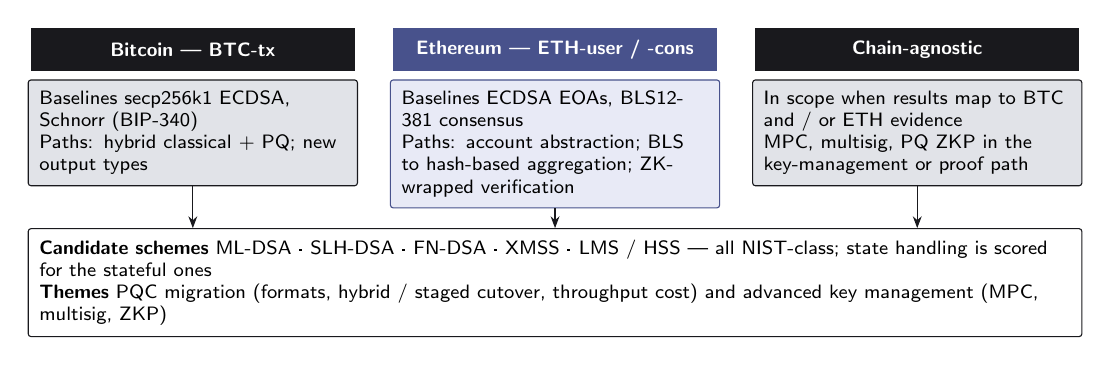
\begin{tikzpicture}[font=\scriptsize, box/.style={draw=bar,fill=lane,rounded corners=1pt,text width=3.9cm,align=left,inner sep=4pt}, hd/.style={fill=bar,text=white,font=\scriptsize\bfseries,text width=3.9cm,align=center,inner sep=3pt,minimum height=5.5mm}]
    \node[hd] (h1) at (0,0) {Bitcoin --- BTC-tx};
    \node[hd,fill=eth] (h2) at (4.6,0) {Ethereum --- ETH-user / -cons};
    \node[hd] (h3) at (9.2,0) {Chain-agnostic};
    \node[box,below=1mm of h1] (b1) {Baselines secp256k1 ECDSA, Schnorr (BIP-340)\\ Paths: hybrid classical + PQ; new output types};
    \node[box,fill=ethbg,draw=eth,below=1mm of h2] (b2) {Baselines ECDSA EOAs, BLS12-381 consensus\\ Paths: account abstraction; BLS to hash-based aggregation; ZK-wrapped verification};
    \node[box,below=1mm of h3] (b3) {In scope when results map to BTC and / or ETH evidence\\ MPC, multisig, PQ ZKP in the key-management or proof path};
    \node[draw=bar,fill=white,rounded corners=1pt,text width=13.1cm,inner sep=4pt,align=left,below=2.5mm of b2.south,anchor=north] (ev) {\textbf{Candidate schemes} ML-DSA \textperiodcentered{} SLH-DSA \textperiodcentered{} FN-DSA \textperiodcentered{} XMSS \textperiodcentered{} LMS / HSS --- all NIST-class; state handling is scored for the stateful ones\\ \textbf{Themes} PQC migration (formats, hybrid / staged cutover, throughput cost) and advanced key management (MPC, multisig, ZKP)};
    \foreach \b in {b1,b2,b3} \draw[-{Stealth[length=1.5mm]},bar] (\b.south) -- (\b.south |- ev.north);
  \end{tikzpicture}
  \end{center}
  {\small Comparative scoring is anchored on Bitcoin and Ethereum. Chain-agnostic work is welcome when it can be mapped to those targets.}
  \takeaway{Japan funds the prize. BGIN turns shared evidence into standards-ready artifacts. NIST remains the reference for which PQC primitives are in scope.}
\end{frame}

% ---------------------------------------------------------------- 10 timeline (drawn; blank in the original PDF)
\begin{frame}{From This Room to the 2028 Award}
  \begin{center}
  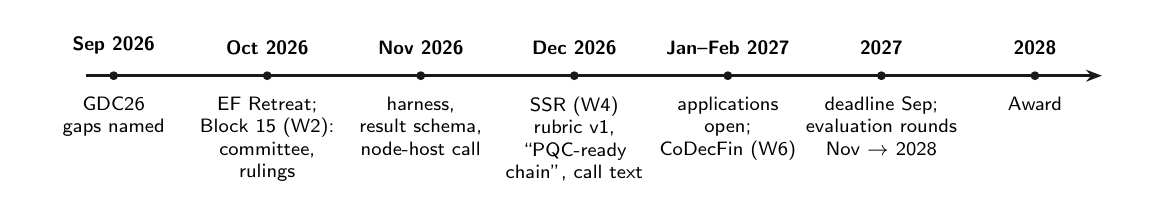
\begin{tikzpicture}[font=\scriptsize]
    \draw[line width=1pt,bar,-{Stealth[length=2mm]}] (0,0) -- (12.9,0);
    \foreach \x/\lab/\txt in {
      0.35/Sep 2026/{GDC26\\ gaps named},
      2.3/Oct 2026/{EF Retreat;\\ Block 15 (W2):\\ committee, rulings},
      4.25/Nov 2026/{harness,\\ result schema,\\ node-host call},
      6.2/Dec 2026/{SSR (W4)\\ rubric v1, ``PQC-ready\\ chain'', call text},
      8.15/Jan--Feb 2027/{applications open;\\ CoDecFin (W6)},
      10.1/2027/{deadline Sep;\\ evaluation rounds\\ Nov $\rightarrow$ 2028},
      12.05/2028/{Award}}
      {\fill[bar] (\x,0) circle (1.6pt);
       \node[above=1.5mm,align=center,font=\scriptsize\bfseries] at (\x,0) {\lab};
       \node[below=1.5mm,align=center,text width=1.95cm] at (\x,0) {\txt};}
  \end{tikzpicture}
  \end{center}
  \par\vspace{1mm}
  \begin{center}\small
    Competition / evaluation $\rightarrow$ BGIN Standard $\rightarrow$ ISO/TC 307 $\rightarrow$ Japan's crypto-asset security criteria
  \end{center}
  {\scriptsize\color{soft} Dates are indicative until the host confirms the call.}
  \takeaway{This 50 minutes can still change what the call asks teams to prove. Block \#15 is the next drafting stop.}
\end{frame}

% ---------------------------------------------------------------- 11 what for
\begin{frame}{What This 50 Minutes Is For}
  \begin{itemize}\small
    \item Document DLT-specific \textbf{deployment gaps} --- activation, wallets, L2, dormant funds, evidence --- rather than re-litigating NIST selections.
    \item Put \textbf{resource estimates} and \textbf{migration design} in the same conversation, so urgency is argued from assumptions, not from slogans.
    \item Name where \textbf{post-quantum ZKP} and \textbf{MPC} change the key-management and proof path, without turning the hour into a ZKP-only session.
    \item Align what policymakers, protocol teams, wallet vendors, and evaluation communities each need to see before they can act.
  \end{itemize}
  \takeaway{The outcome is a short list of gaps and Block \#15 decisions --- not a locked migration spec tonight.}
\end{frame}

% ---------------------------------------------------------------- 12 discussion items
\begin{frame}{Discussion Items for This Room}
  \begin{enumerate}\small
    \item Which objects move first: long-lived confidentiality under harvest-now / decrypt-later, on-chain signatures that must remain verifiable, or the proof and key-management path (PQ ZKP, MPC)?
    \item What would make a \textbf{resource estimate} usable for a policymaker --- assumptions, error bars, and what must not be collapsed into a Q-day date?
    \item What must a \textbf{neutral testbed} measure so that ``PQ-ready'' is comparable across stacks?
    \item How should \textbf{crypto agility} be specified so wallets and ST/PP profiles can rotate algorithms without a fork-by-fork rewrite?
  \end{enumerate}
\end{frame}

% ================================================================ NEW: notes for the Ethereum community
% ---------------------------------------------------------------- 13 section divider
{\setbeamertemplate{footline}{}
\begin{frame}[plain,t]
  \begin{tikzpicture}[remember picture,overlay]
    \fill[eth] (current page.north west) rectangle ([yshift=-3.1cm]current page.north east);
    \node[anchor=north east,inner sep=0] at ([xshift=-7mm,yshift=-5mm]current page.north east){
\includegraphics[height=1.9cm]{bgin_logo.png}};
    \node[anchor=west,text=white,font=\Large\bfseries] at ([xshift=7mm,yshift=-1.55cm]current page.north west){Notes for the Ethereum Community};
    \node[anchor=west,text=white,font=\small,text width=11.2cm,align=left] at ([xshift=7mm,yshift=-2.35cm]current page.north west){Taking part in Japan's PQC Migration Prize};
    \node[anchor=west,font=\small,text width=14cm,align=left] at ([xshift=7mm,yshift=-4.4cm]current page.north west){Ethereum is one of the two evidence anchors of the competition, on both the user layer and the consensus layer. The evaluation design is still in draft, and the people who build Ethereum can still shape what entrants are asked to prove.};
    \node[anchor=west,font=\scriptsize,text=soft,text width=14cm,align=left] at ([xshift=7mm,yshift=-5.9cm]current page.north west){Source for every fact on the next three slides: github.com/bgin-global/pqc-agility-competition (draft v0; nothing is ratified until the evaluation committee adopts it). Nothing here asks Ethereum to adopt anything.};
  \end{tikzpicture}
\end{frame}}

% ---------------------------------------------------------------- 14 where ethereum sits / what is measured
\begin{frame}{Where Ethereum Sits --- and What the Testbed Measures}
  \ethlead{Two Ethereum evidence classes are scored, plus an L2 class: \textbf{ETH-user} (EOA and account-abstraction signatures, on-chain verification cost) and \textbf{ETH-cons} (validator BLS aggregation and its hash-based successors).}
  \begin{center}\scriptsize
  \begin{tabular}{@{}>{\raggedright\arraybackslash}p{1.3cm}>{\raggedright\arraybackslash}p{4.2cm}>{\raggedright\arraybackslash}p{8.1cm}@{}}\toprule
    \textbf{Class} & \textbf{Baseline and paths} & \textbf{Candidate metrics (scored against the classical baseline)}\\ \midrule
    ETH-user & ECDSA secp256k1 EOAs; hybrid classical + PQ; account-abstraction path & Calldata bytes and gas at a reference block mix; on-chain verification gas, precompile \emph{and} contract path; gossip propagation p50 / p95; block validation delta; state bytes per account; wallet and hardware-wallet impact\\
    ETH-cons & BLS12-381 aggregation; BLS to hash-based aggregation & Batch / aggregate verify throughput at 1 to 100{,}000 signers; aggregate signature size; block validation delta\\
    L2 & ZK-wrapped verification (prove many PQ signatures, verify one proof) & Constraints or prover seconds to verify one signature in a reference proof system\\ \bottomrule
  \end{tabular}\end{center}
  {\footnotesize Shared by every class: migration throughput, rollback cost, agility switch cost, legacy verification continuity, reproducibility, security review, governance fit.}
  \ethnote{Entries are judged on evidence mapped to these classes. Ethereum-native methods make the scores meaningful to client teams.}
\end{frame}

% ---------------------------------------------------------------- 15 open rulings
\begin{frame}{Open Rulings the Ethereum Community Can Shape}
  \ethlead{Every integration path is a committee ruling, not a default. These open items carry the most Ethereum weight; rulings start at Block 15 (W2).}
  \begin{enumerate}\footnotesize\setlength{\itemsep}{0.5mm}
    \item \textbf{Hash-based aggregation parameters.} Consensus-layer work is heading toward XMSS-style aggregation with Poseidon2 for ZK-friendliness. That parameterization sits outside NIST SP 800-208, so its admission needs an explicit ruling.
    \item \textbf{One rubric or two.} Are consensus-layer and user-level evidence scored on one rubric or on separate ones?
    \item \textbf{Reference workload.} Which reference block mix and which reference CPU class anchor the gas, calldata and validation-time metrics?
    \item \textbf{Account abstraction.} How the precompile path and the contract-verification path are both reported, so gas numbers are comparable.
    \item \textbf{Proof systems.} Which reference post-quantum proof system anchors the ZK-wrapped verification metric.
    \item \textbf{Burden split.} Who upgrades first, node operators or users, and how migration throughput reflects that.
  \end{enumerate}
  \ethnote{The Quantum Retreat outputs (Cambridge, 9--12 Oct) are a listed resource for these rulings. Bring them to Block 15.}
\end{frame}

% ---------------------------------------------------------------- 16 how to take part
\begin{frame}{How Ethereum Teams Can Take Part}
  \ethpillar{0.31\textwidth}{Shape it (Autumn 2026)}{\begin{itemize}\scriptsize
    \item \textbf{Evaluation committee:} 2--3 Ethereum developer / project seats, named a primary evaluation focus. Nominate by issue template, with a conflict-of-interest disclosure.
    \item \textbf{Technical advisor:} Ethereum-track input without winner-selection votes.
    \item \textbf{Metric or scheme proposal:} an issue, then a pull request to the metric register or scheme list.
  \end{itemize}}\hfill
  \ethpillar{0.31\textwidth}{Measure it (2026--2028)}{\begin{itemize}\scriptsize
    \item \textbf{Testbed node host:} a university or neutral lab runs a BSafe.network evaluation node. Hosting is kept separate from judging.
    \item \textbf{Calibration tracks:} propose an Ethereum track, or submit to an open one; results are promoted only by independent reproduction.
  \end{itemize}}\hfill
  \ethpillar{0.31\textwidth}{Enter it (2027)}{\begin{itemize}\scriptsize
    \item \textbf{Submit:} Ethereum developers and project teams are a primary entrant group. Applications planned to open January 2027; deadline planned September 2027.
    \item \textbf{Workshops:} Block 15 (Oct), SSR Baltimore (13 Dec, call text), CoDecFin at FC'27 (Feb).
  \end{itemize}}
  \par\vspace{2mm}
  {\small Conversation: the \emph{Post-Quantum Crypto Agility Competition} category on bgin.discourse.group. Record: the repository. Every commit there is signed and carries a DCO sign-off.}
  \ethnote{Planning to submit does not bar a seat. It is disclosed, and submitters do not judge their own round; node hosts do not measure their own artifact.}
\end{frame}

% ================================================================ original deck resumes
% ---------------------------------------------------------------- 17 discussion starter title
{\setbeamertemplate{footline}{}
\begin{frame}[plain,t]
  \begin{tikzpicture}[remember picture,overlay]
    \fill[bar] (current page.north west) rectangle ([yshift=-3.1cm]current page.north east);
    \node[anchor=north east,inner sep=0] at ([xshift=-7mm,yshift=-5mm]current page.north east){
\includegraphics[height=1.9cm]{bgin_logo.png}};
    \node[anchor=west,text=white,font=\Large\bfseries] at ([xshift=7mm,yshift=-1.55cm]current page.north west){Why a TLS Playbook Will Not Migrate This Stack};
    \node[anchor=west,text=white,font=\small,text width=11.2cm,align=left] at ([xshift=7mm,yshift=-2.35cm]current page.north west){A working frame for this breakout};
    \node[anchor=west,font=\normalsize] at ([xshift=7mm,yshift=-4.5cm]current page.north west){Shin'ichiro Matsuo, Ph.D.};
    \node[anchor=west,font=\small,text=soft] at ([xshift=7mm,yshift=-5.15cm]current page.north west){BGIN Co-Chair \textbar{} Breakout: PQC Migration on DLTs};
    \node[anchor=west,font=\small,text=soft] at ([xshift=7mm,yshift=-5.65cm]current page.north west){Global Digital Collaboration \textbar{} Geneva \textbar{} 2--3 September 2026};
    \node[anchor=west,font=\scriptsize,text=soft] at ([xshift=7mm,yshift=-6.5cm]current page.north west){Discussion starter};
  \end{tikzpicture}
\end{frame}}

% ---------------------------------------------------------------- 18 writing problem
\begin{frame}{The writing problem is not a missing algorithm}
  \lead{NIST already standardized the first primitives. Adjacent Internet protocols already have hybrid patterns. The BGIN job is not a rival scheme.}
  {\small For public ledgers and wallets, migrating in a way that a community can actually run is hard for three stacked reasons:}\par\vspace{1.5mm}
  \pillar{0.31\textwidth}{Public verification}{Keys and signatures often sit in the clear. Harvest-now is not only an archival problem.}\hfill
  \pillar{0.31\textwidth}{Consensus freeze}{Validity rules are global. You cannot negotiate a cipher suite per connection the way TLS does.}\hfill
  \pillar{0.31\textwidth}{Economic incentives}{Dormant funds, wallet UX, miner and custodian costs, and multi-client stacks decide whether a clean design ships.}
  \takeaway{Design for the next migration now. A rushed cutover creates new incidents; a frozen profile goes stale.}
\end{frame}

% ---------------------------------------------------------------- 19 at-rest vs on-spend
\begin{frame}{At-Rest versus On-Spend --- Timing Is Not One Number}
  \lead{Shor recovers signing keys from exposed public keys. When the public key appears on-chain changes when the attack becomes live.}
  \pillar{0.48\textwidth}{At-rest}{The public key is already on-chain. An adversary can grind offline against a stored verification key until a cryptographically relevant quantum computer can forge spends.}\hfill
  \pillar{0.48\textwidth}{On-spend}{The public key is revealed only when funds move. The race is then between the legitimate owner and an attacker who sees the broadcast, not an unbounded offline grind.}
  \par\vspace{1.5mm}
  {\small Address design, reuse, and wallet defaults therefore change the threat model. A single Q-day slogan erases that difference.}
  \takeaway{Resource estimates only become policy-useful when they are tied to which keys are already public.}
\end{frame}

% ---------------------------------------------------------------- 20 questions
\begin{frame}{Questions for this room}
  \lead{This 50-minute breakout is for mapping gaps and naming what Block \#15 must decide --- not for locking a first migration spec tonight.}
  \begin{enumerate}\small
    \item Which \textbf{objects} should BGIN triage first, and which can wait: at-rest keys, on-spend paths, credentials, PQ ZKP, MPC?
    \item What would make a \textbf{resource estimate} honest enough for this audience --- and what language should we refuse (single Q-day, vendor screenshots)?
    \item What must a \textbf{neutral evaluation} see so that hybrid then cutover is comparable across Bitcoin-class, account-model, and wallet stacks?
    \item How should agility be written so ST/PP and wallet profiles can \textbf{rotate} without forking the scheme every time the primitive list moves?
  \end{enumerate}
\end{frame}

% ---------------------------------------------------------------- 21 join
\begin{frame}{Join us at BGIN Block 15}
  \lead{15--16 October 2026 \textbar{} Georgetown University Capitol Campus, 111 Massachusetts Ave NW, Washington, D.C. \textbar{} In person (remote available). The PQC drafting and measurement work listed above continues in the Block 15 IKP sessions.}\vspace{-1.5mm}
  {\small\textbf{Related sessions}}
  \begin{itemize}\small
    \item 15 Oct, 09:20--09:50 (Room A). Keynote: PQC
    \item 15 Oct, 09:50--11:20 (Room B). IKP: PQC Migration (1) --- resource estimates into judging criteria
    \item 15 Oct, 11:30--13:00 (Room B). IKP: PQC Migration (2) --- crypto agility and the NIST signature migration, with NIST participation
  \end{itemize}
  \par\vspace{-1mm}
  \begin{center}\tiny
    \begin{tabular}{@{}>{\centering\arraybackslash}p{3.1cm}@{\hspace{2mm}}>{\centering\arraybackslash}p{3.1cm}@{\hspace{2mm}}>{\centering\arraybackslash}p{3.1cm}@{\hspace{2mm}}>{\centering\arraybackslash}p{3.1cm}@{}}
      \qrcode[height=1.25cm]{https://bgin-global.org/events/20261015-block15/sessions/1-4} &
      \qrcode[height=1.25cm]{https://bgin-global.org/events/20261015-block15} &
      \qrcode[height=1.25cm]{https://www.eventbrite.com/e/bgin-block15-tickets-1990274282957} &
      \qrcode[height=1.25cm]{https://github.com/bgin-global/pqc-agility-competition} \\[0.5mm]
      \textbf{PQC session} & \textbf{Block 15 site} & \textbf{Register} & \textbf{Competition repo} \\
      bgin-global.org/events/ 20261015-block15/sessions/1-4 & bgin-global.org/events/ 20261015-block15 & eventbrite.com/e/ bgin-block15-tickets & github.com/bgin-global/ pqc-agility-competition
    \end{tabular}
  \end{center}
  \takeaway{Hybrid. Connection details are sent after registration. You are invited.}
\end{frame}

\end{document}
